%%
%% Introduction:
%% A paper about using GeoHash to control the epidemic
%% Use covid-19 as example
%% Youwei Huang
%% IICT, CAS
\documentclass[sigplan,screen]{acmart}

\usepackage{subfigure}
\usepackage{gensymb}
\usepackage{algorithm}
\usepackage{algorithmicx}
\usepackage{algpseudocode}
\renewcommand{\algorithmicrequire}{\textbf{Input:}}
\renewcommand{\algorithmicensure}{\textbf{Result:}}

\begin{document}
\title{Epidemic Prevention and Control Based On GeoHash}

\author{Youwei Huang}
\email{huangyw@iict.ac.cn}
\affiliation{%
	\institution{Institute of Intelligent Computing Technology, Chinese Academy of Sciences}
	\city{Suzhou}
	\country{China}
}

\author{Feng Lu}
\email{lufeng20g@ict.ac.cn}
\affiliation{%
	\institution{Institute of Computing Technology, Chinese Academy of Sciences}
	\city{Beijing}
	\country{China}
}

\begin{teaserfigure}
	\centering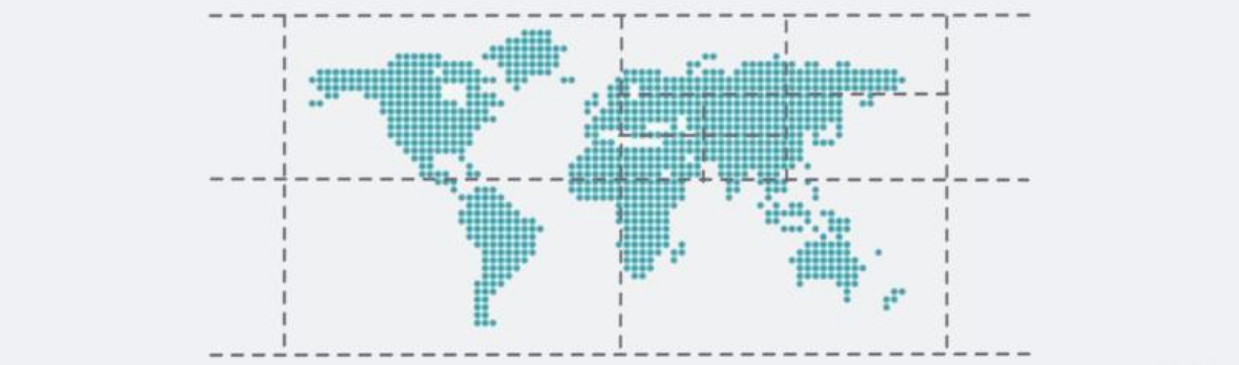
\includegraphics[width=\linewidth]{logo.png}
	\caption{GeoHash for geographic grid division}
	\Description{In 2008, Gustavo Niemeyer invented GeoHash which can encode a geographic position into a short string}
\end{teaserfigure}

\begin{abstract}
	COVID-19 (Coronavirus Disease 2019) which is a contagious disease caused by SARS-CoV-2\cite{hu2020characteristics} was first detected in Dec. 2019.
	Until 2021, the virus is still spreading over the world.
	Before the vaccine is widely used or the invention of specific medication, many measures have been taken by people to prevent the spread of the epidemic.
	In such an emergency period, we have to quarantine the high-risk groups and lock down the seriously infected regions.
	We propose a kind of dynamic block division technology based on \textbf{GeoHash} used to monitor, screen and control the epidemic areas.
	\textbf{GeoHash} is a public domain geocode system invented in 2008 by Gustavo Niemeyer\cite{niemeyer2008geohash}.
	We divide the world into several scaleable blocks by using \textbf{GeoHash}.
	Through \textbf{GIS}, these blocks can be easily visualized on the digital map of any electronic device.
	A map generated by \textbf{GIS} which is used for epidemic prevention and control can be named as \textbf{``Epidemic Map''}.
	Each of the blocks on \textbf{Epidemic Map} contains epidemic information and other important characteristics which are concerned by medical work.
	Blocks are scaleable and cover on the map as regular geometric shapes.
	In this way, we carry out quantitative analysis of epidemic data on each block.
	The results of analysis support for decision-making, measures formulation, and effectiveness assessment of COVID-19 prevention and control.
	Such a geographic information system applies not only to COVID-19, but also to other epidemic diseases.
\end{abstract}
\keywords{GeoHash, COVID-19, GIS, big data, epidemic prevention and control}

\maketitle
\section{Introduction}
During the COVID-19 pandemic, many cities over the world were forced to lock down.
Wuhan City and the major cities in Hubei, China were put under lockdown on the 23rd and 24th of January, respectively\cite{lau2020positive}.
Lockdown meant the whole region was quarantined and cut off physical contact with the outside world.
The citizens were forbidden to leave their city or even their home.
The national medical team carried out centralized medical observation and treatment in quarantined cities.
Research shows, COVID-19 spread became weaker following lockdown\cite{lau2020positive}.
However the lockdown of a city can cause huge economic losses.
The lockdown of some vital areas can cause irreparable losses, such as financial center, political center, and industrial dependent cities.
Another issue that confuses people is how to distinguish whether the area they are in or where they are going is safe.
The current regional risk warning or lockdown is based on the administrative divisions as Figure 2.
Cities, states or provinces all over the world have different sizes and irregular geographic borders.
There may be an outbreak in a city, but it does not mean that the virus has spread to all corners of the city.
On the contrary, there may be no epidemic in the center of neighboring cities, but there is already a huge risk at the border of these cities.
Figure 2 is a map that shows the initial locked down cities in Hubei province, China, a white block surrounded by red blocks was dangerous, even if it was not locked down at that time.
\begin{figure}[htb]
	\centering
	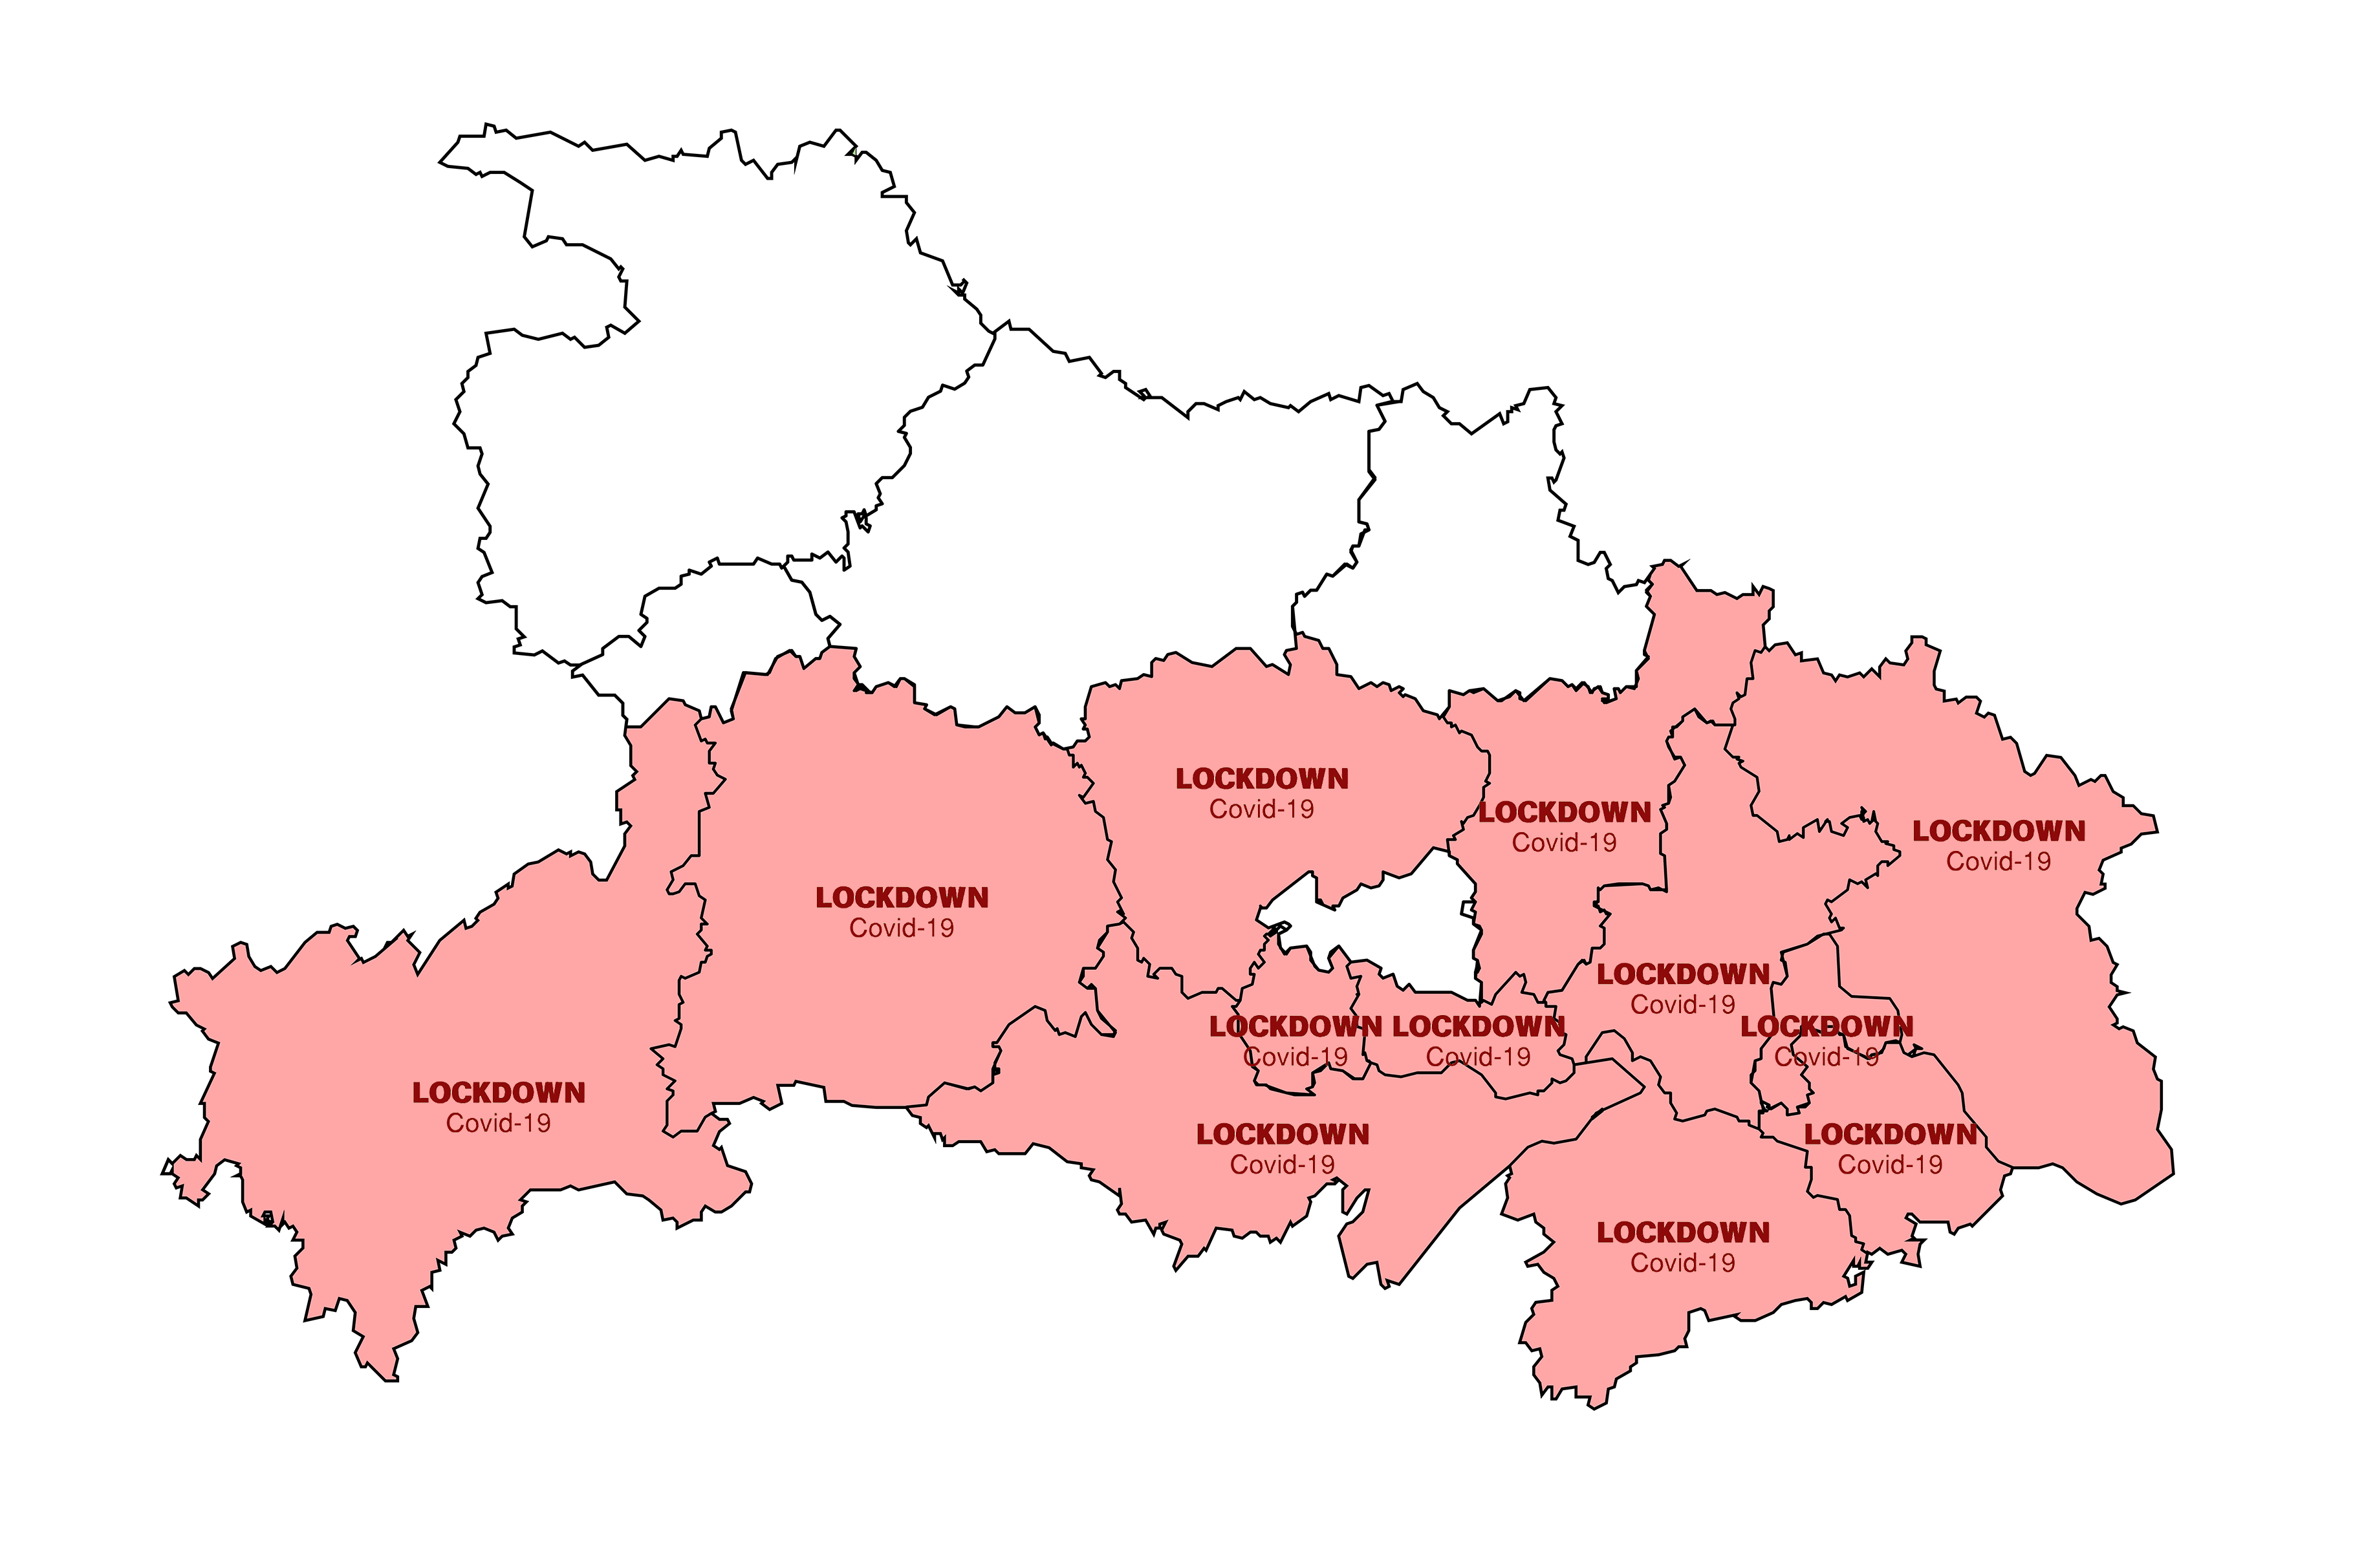
\includegraphics[width=\linewidth]{hubei.png}
	\caption{Map of locked down administrative divisions of Hubei province in China. [Public domain], via Wikipedia. (\url{https://en.wikipedia.org/wiki/COVID-19_lockdown_in_Hubei}).}
	\Description{Locked down cities in Hubei province, white color are unlocked cities and red color are locked cities.}
\end{figure}
\\
We summarize some main weaknesses by taking the current prevention and control measures:
\begin{enumerate}
	\item The border of a city is irregular and the transmission of virus doesn't follow the administrative division, so the lockdown is not accurate.
	\item The administrative size of a city is fixed, but the disease is spreadable, so the lockdown is not expanded flexibly.
	\item Due to policy differences in different regions, information release is not complete and uniform.
	\item The news released by local government can be lagging and residents are hard to get the news in real time.
\end{enumerate}
Based on the above statements, it is not the best way to observe and control the epidemic area through the administrative division.
For infectious diseases, we have abandoned the common administrative control methods.
We have adopted a technology based on GIS (Geographic Information System)\cite{clarke1986advances}.
\textbf{GeoHash} is used to divide map into several geometric blocks.
The 2-dimensional geometric blocks on map are encoded by \textbf{GeoHash}, so they are reduced to 1-dimension and stored as strings in database.
These blocks are presented as regular geometry, but can be scaled according to the needs of different observation scope.
\\
Meanwhile, we do this technology is because it has the following advantages:
\begin{enumerate}
	\item The blocks divided by GeoHash are regular geometry, and the shape can be customized by observer.
	\item The blocks are generated dynamically and they are scalable according to the scope of infection.
	\item Information of the epidemic can be encoded in GeoHash or directly saved.
	\item Block data can be quantified in GIS, as example of generating safety index.
	\item When such a GIS is released to the Internet, users get epidemic information in real time.
\end{enumerate}
In the practical and experimental scenarios, we use mobile application and web technology to develop such a GIS for medical prevention and treatment as shown in Figure 3.
It works for medical workers as a visual auxiliary tool and share with users the results of epidemic data analysis in real time.
The \textbf{ASI} in Figure 3 is a value of ``Area Safety Index'', which is the focus of this paper.
\textbf{ASI} represents the risk level of a region.
The system contributes to enlighten and support decisions of governments, medical institutions, residents, and other researchers who are concerned about the epidemic.
\\
The core idea of this paper is to divide the earth to blocks. Blocks have the following characteristics:
\begin{enumerate}
	\item Blocks are regular geometry neighboring with each other.
	\item Blocks can be scaled on the map.
	\item Blocks are created only when they are meaningful.
	\item Scaling is limited, with the smallest and largest block size.
	\item Blocks scaling levels are discrete sizes, not continuous.
	\item Blocks store structured data, which can be used for the data analysis.
\end{enumerate}
The last item in the above list indicates that the purpose of dividing to blocks is to perform quantitative analysis of the epidemic situation.
\\
We will also introduce other related work in controlling epidemic by using the similar information technology and computer visualization technology.
The paper will mainly focus on how to use \textbf{GeoHash} to divide blocks, and explain the methods of quantifing epidemic data on \textbf{GeoHash} blocks.

\begin{figure*}[hptb]
	\centering{
		\subfigure[larger scale]{
			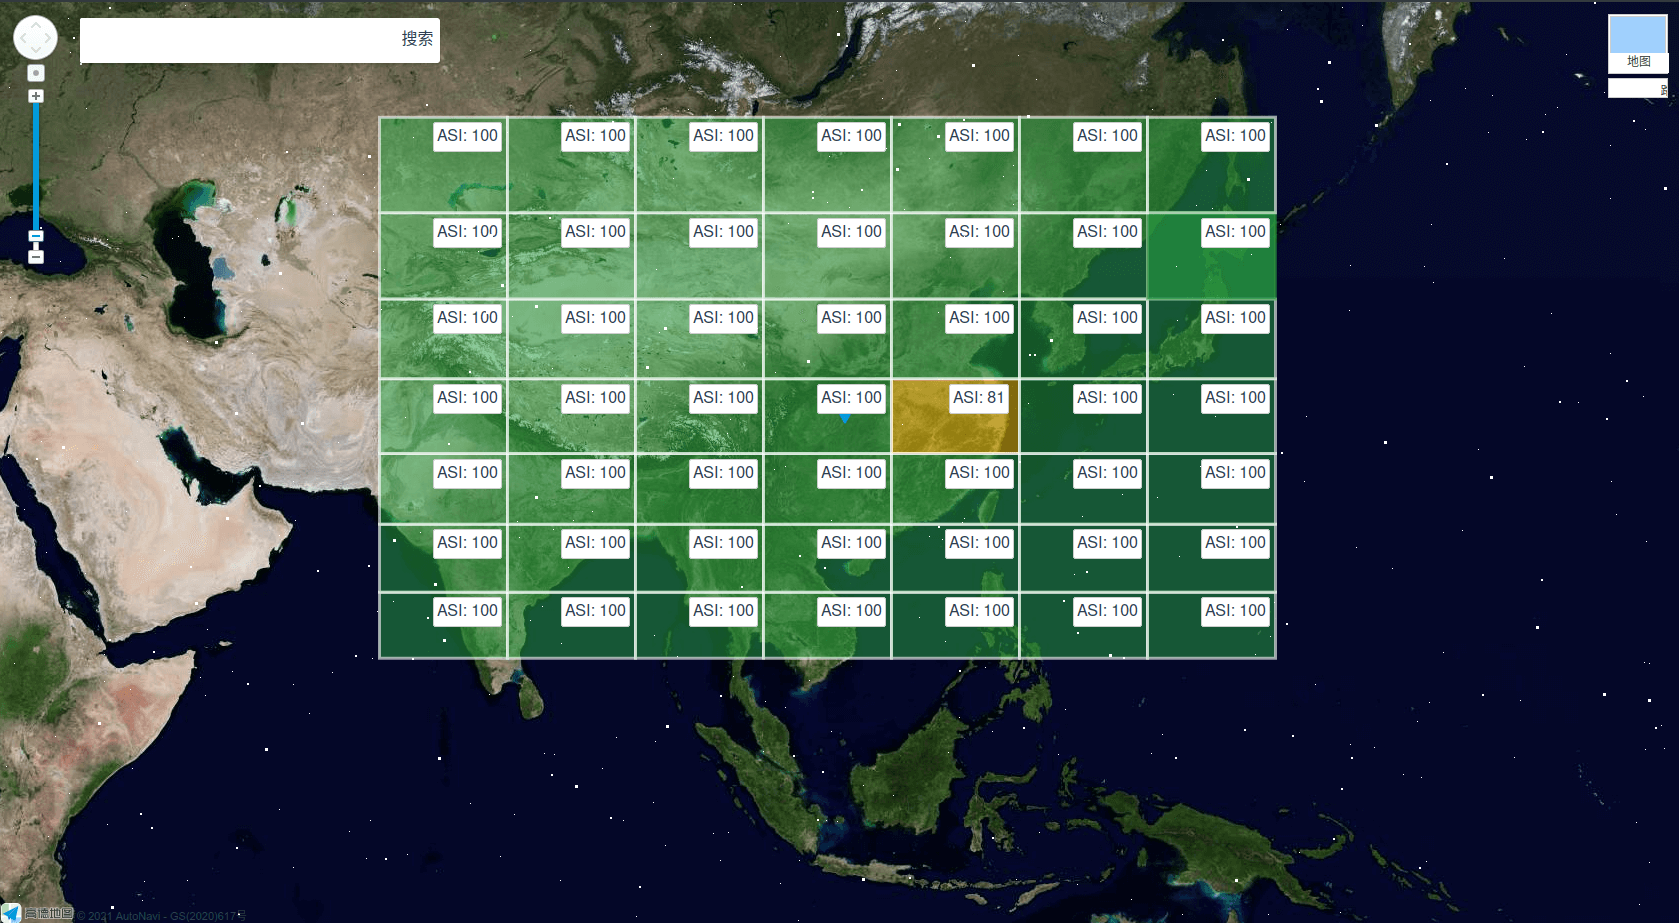
\includegraphics[width=\textwidth]{geogrids1.png}
		}
		\subfigure[smaller scale]{
			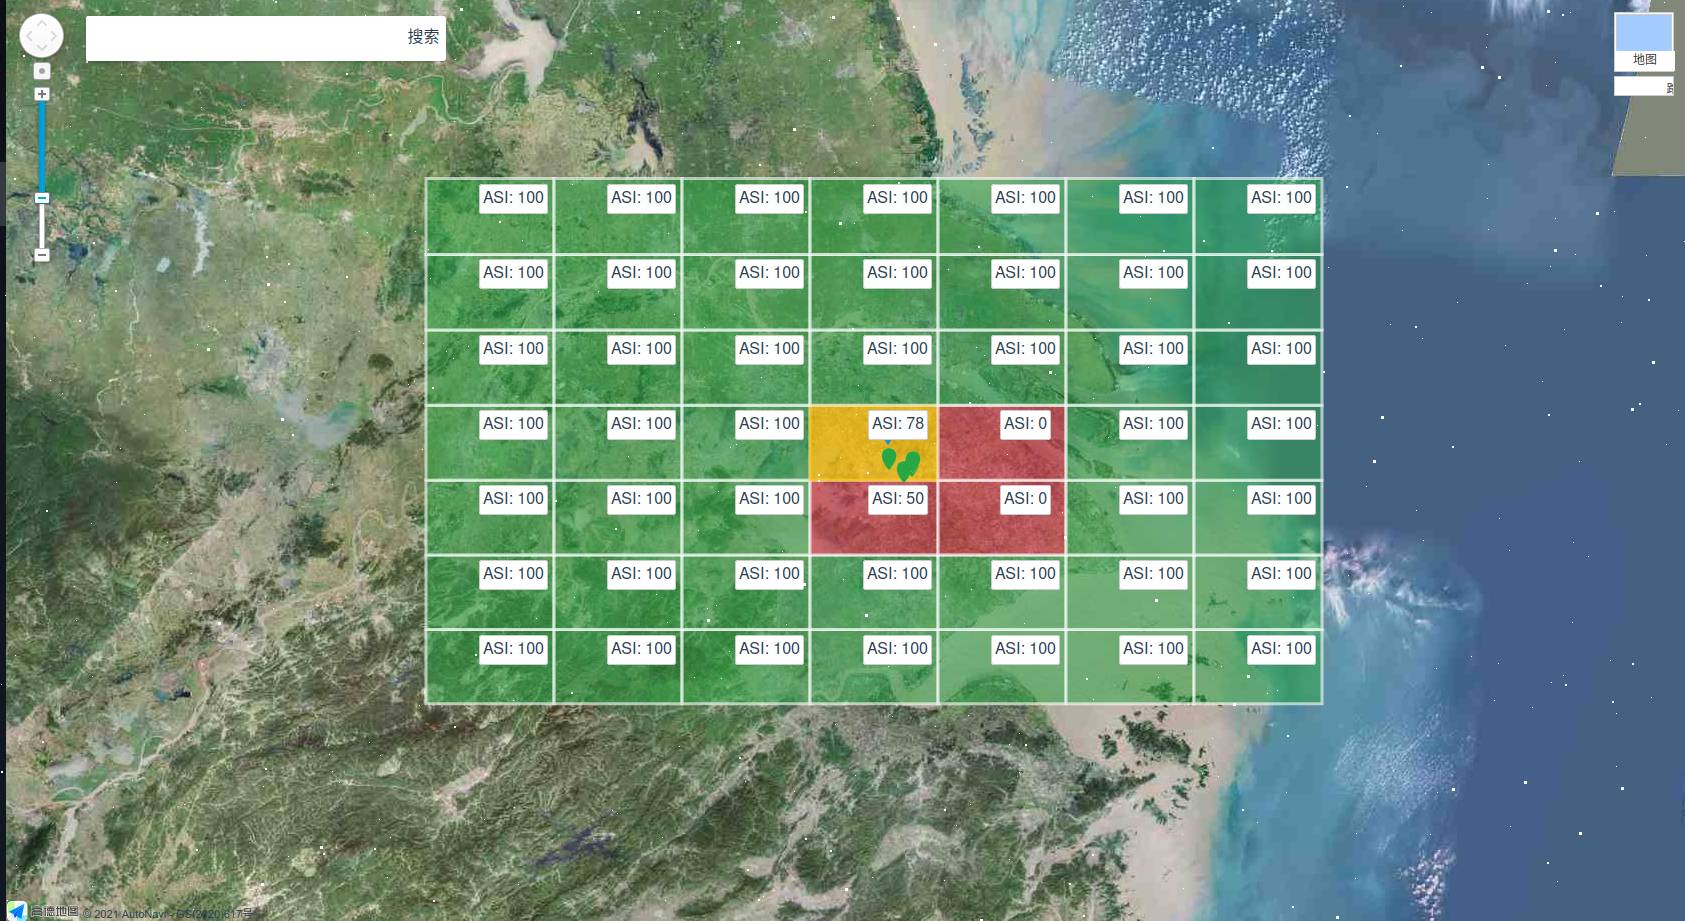
\includegraphics[width=\textwidth]{geogrids2.png}
		}
		\caption{Dynamic blocks in geographic information system}
	}
\end{figure*}

\section{Related Work}
There are some mature cases of controlling and treating COVID-19 pandemic by using information system and data visualization technology.
Many studies on COVID-19 have recently emerged, and various data science applications combating the pandemic have been reported recently\cite{latif2020leveraging}.
The main functions of these systems or softwares are listed as follows:\cite{jia2020big}
\begin{itemize}
	\item Tracking of people's movements.
	\item Early warning of high-risk areas.
	\item Screening of asymptomatic potential infections.
	\item Drug development.
	\item Information release and policy support.
\end{itemize}
\subsection{Data Visualization Analysis}
Visualization technology presents data to users by drawing charts and graphics, in which the data is represented by symbols, such as bar charts, line charts, pie charts, maps and etc\cite{jensen1992harvard}.
\begin{figure}[htb]
	\centering
	\subfigure[Choropleth Map]{
		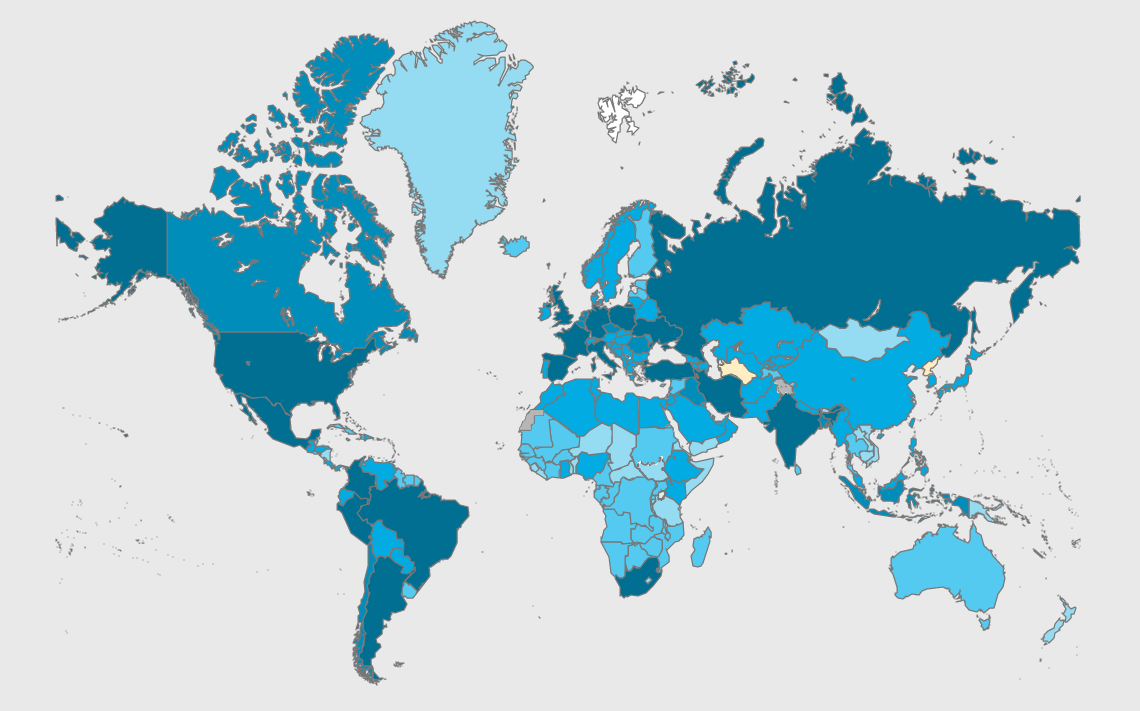
\includegraphics[width=\linewidth]{worldmap1.png}
	}
	\subfigure[Bubble Map]{
		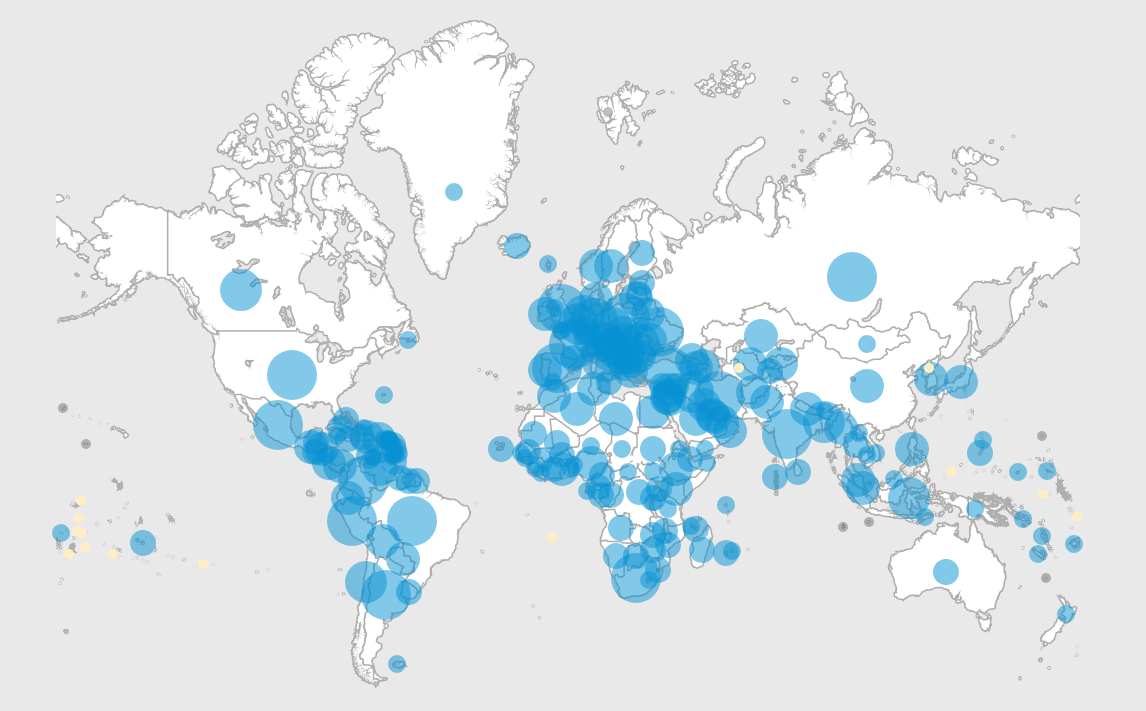
\includegraphics[width=\linewidth]{worldmap2.png}
	}
	\caption{WHO coronavirus disease dashboard. [Public domain], via WHO (\url{https://covid19.who.int})}
	\Description{The figures are captured from the official website of WHO, the web page uses a dashboard to show the COVID-19 situation over the world.}
\end{figure}
\\
Figure 4 shows the global COVID-19 epidemic situation in the form of map charts. The epidemic maps are updated by WHO (World Health Organization)\footnote{https://www.who.int} in real time, to display the number of cases around the world.
\\
Maps in Figure 4 uses two styles of presentation: choropleth and bubble.
One uses the depth of color to show the severity of the epidemic situation in each country, and another uses the bubble size to show the number of infections.
No matter what kind of map, its role is to help the local people easy to understand the severity of the epidemic, and prompt the local government to take actions to treat and control the epidemic situation.
These two figures in Figure 4 are similar to the previous Figure 2, except that Figure 2 only shows one province.
Contents in these maps include like: confirmed cases, deaths, historical cases, added cases, regional lockdown status, and etc.
Some weaknesses of such kind of maps are discussed in the introduction section (Section 1).
\\
The bar charts and line charts are aslo widely used in epidemic data analysis.
These graphs are mostly used to show the trend of epidemic situation and transmission cycle.
Figure 5 showws an example that uses both bar chart and line chart to perform the trend of daily new cases from Jan. 2020 to Jan. 2021 in the United States.
The red line in this chart is the 7-day moving average curve.
Other trends from different types of data, such as death trends, can be found on the official CDC\footnote{https://covid.cdc.gov/covid-data-tracker} website.
\begin{figure}[htb]
	\centering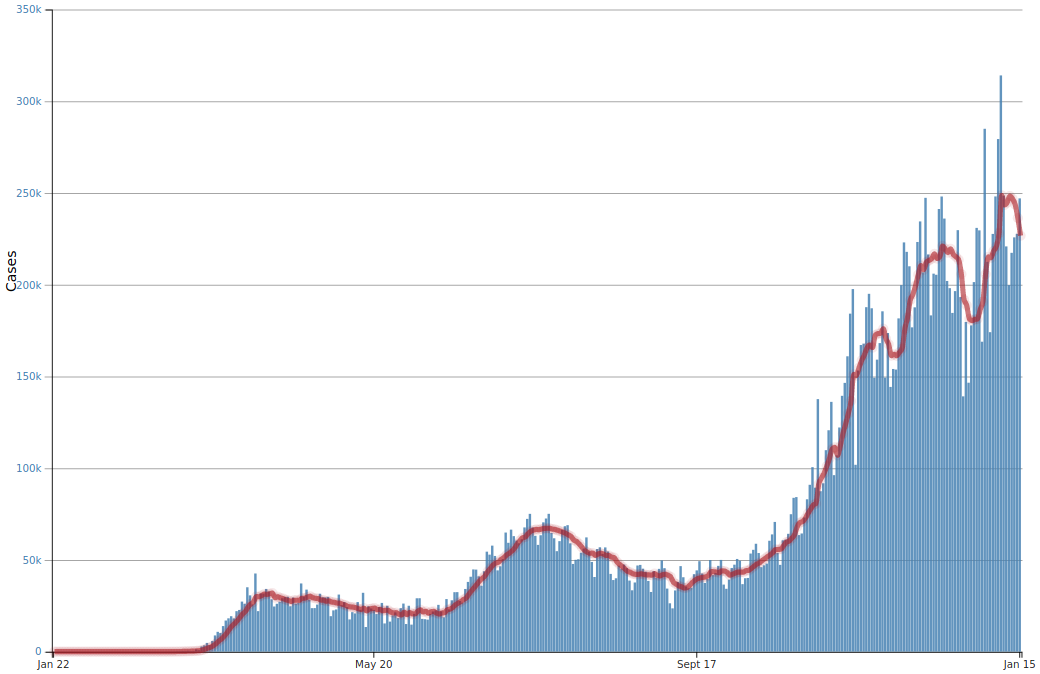
\includegraphics[width=\linewidth]{linebar-us-1-15.png}
	\caption{Daily trends in number of COVID-19 new cases in the US reported to CDC. [Public domain], via CDC (\url{https://covid.cdc.gov/covid-data-tracker/\#trends_dailytrendscases})}
	\Description{The figure is a screenshot from CDC official web page, it shows the daily new cases in the US by drawing a bar and line chart.}
\end{figure}
\\
The line charts and bar charts reflect historical epidemic data from time series, while map charts reflect epidemic data from spatial distribution.
In other related work survey, visual data analysis are used to study the relationship between population mobility and the epidemic spreading pattern.
During the early outbreak of coronavirus in Wuhan, China, the graphs in a research suggested that the number of confirmed cases in other provinces were directly proportional to the inflow of Wuhan population.
The research group also used the pattern derived from the data analysis to predict the number of infections.\cite{chen2020data}
\subsection{Geographic Information System}
The maps we described in the previous section are charts, the information carried by map charts is limited, unflexible, not automatic analysis and not real-time.
Although charts can provide visual perception, users need to analyze the graphs by themselves, but GIS can integrate analysis, prediction and other practical functions.
A GIS (geographic information system) is a conceptualized framework that provides the ability to capture and analyze spatial and geographic data\cite{clarke1986advances}.
Since the outbreak of the epidemic, a number of geographic information systems have been built or have added real-time epidemic related functions, such as ``epidemic map displays'', ``fever clinic queries'' and ``passenger information queries''.
Based on existing commercial GIS softwares, they made important contributions to epidemic prevention and control\cite{zhou2020covid}.
Some of the systems have the function of dynamic zoom map, which can display the situations of different scaling areas, from state level to community level.
For example, Figure 6 shows a map with an epidemic layer on it, it is a GIS tool that shows critical information about COVID-19 cases in an area so the users can make more informed decisions about where to go.
\begin{figure}[htb]
	\centering
	\subfigure[State Level]{
		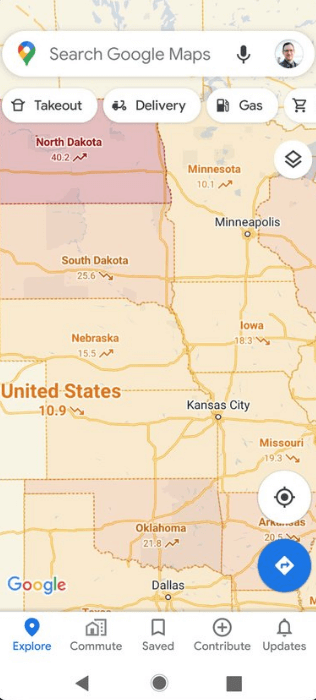
\includegraphics[width=0.45\linewidth,height=80mm]{state-level.png}
	}
	\subfigure[County Level]{
		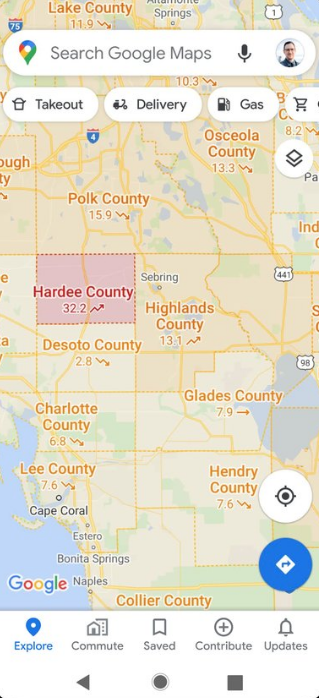
\includegraphics[width=0.45\linewidth,height=80mm]{county-level.png}
	}
	\caption{COVID layer in Google Map of different scales}
\end{figure}
\\
In Figure 6, \textbf{Google Map} adds a COVID-19 layer to the GIS, it also quantities an safety index by using the 7-day average for the number of new cases per 100,000 people.
It also indicates whether cases are increasing or decreasing.
The layer's colors indicate:\footnote{https://support.google.com/maps/answer/9795160}
\begin{itemize}
	\item Grey: Less than 1 case.
	\item Yellow: 1 to 10 cases.
	\item Orange: 10 to 20 cases.
	\item Dark orange: 20 to 30 cases.
	\item Red: 30 to 40 cases.
	\item Dark red: 40 more cases.
\end{itemize}
Unlike \textbf{Google Map}, we perform the quantitative analysis based on dynamic \textbf{GeoHash} blocks instead of administrative regions.
The safety quantification algorithm we use not only includes the simple infected cases.
In the following chapters, we will focus on our research work about how to use \textbf{GeoHash} to improve the GIS in epidemic prevention and control.

\section{Pre-Work}
Our challenges are mainly from two aspects: data collection and data quantification.
Data collection is integrated in GIS, which requires users' devices to upload positions, and the server needs to store the position data submitted by users.
Quantitative analysis of data is a more complex process and our work is to quantify the collected messy data in \textbf{GeoHash} blocks.
\\
For data collection, the system can provide a mobile application for users to view the surrounding epidemic situation.
At the same time, in order to obtain the surrounding epidemic safety situation, users need to upload their own GPS information.
Under the privacy policy, we only collect users' GPS information, but we will not save users' personal informationa. So we don't track or monitor users' positions in the system.
This method of collection is carried out anonymously, and each record is stored as a virtual and unknown identity which means only users know their own locations but other users cannot get it.
\\
After the diagnosis, the medical workers mark the confirmed cases through their virtual identities.
Other users don't know these users' real identity, but they can browse the surrounding infection.
The medical workers know their patients' real identities, but they cannot track their location information without user authorization.
To be simple, our solution is to use the virtual identity or encode user information to separate location information and real user information.
This is an approach to keep a balance between keeping user privacy and collecting data for epidemic control.
\\
For example, in China, a kind of QR code carried by users called \textbf{Health Code} shows one's health status but doesn't tell one's information.
Each QR code corresponds to a unique user in the real world.
In the real world, people use the health code to know the health status of themselves or others.
\\
For data quantification, we need to divide the map to blocks first by using \textbf{GeoHash}.
At the step of GPS data collection, we get the longitude and latitude values from the user.
\textbf{GeoHash} will calculate which block the user belongs to.
Suppose a \textbf{GeoHash} block as a set $B_1$ that includes many users, we quantify the safety index of $B_1$ based on confirmed cases and the total number of the user.
The historical users, ``visitors'' in a block also need to be considered.
These visitors who are diagnosed in the short term will have negative effects on a block.
As discussed above (in Section 2.1), a research has proposed that the number of people infected in a region is positively correlated with the inflow of the population from high-risk areas.
That means, when collecting position data, we noy only need to save user current position, but also need to save user historical location data.
The general storage and calculation process is shown in Figure 7, and the detailed methods and algorithms are described in Section 4.
\begin{figure}[htb]
	\centering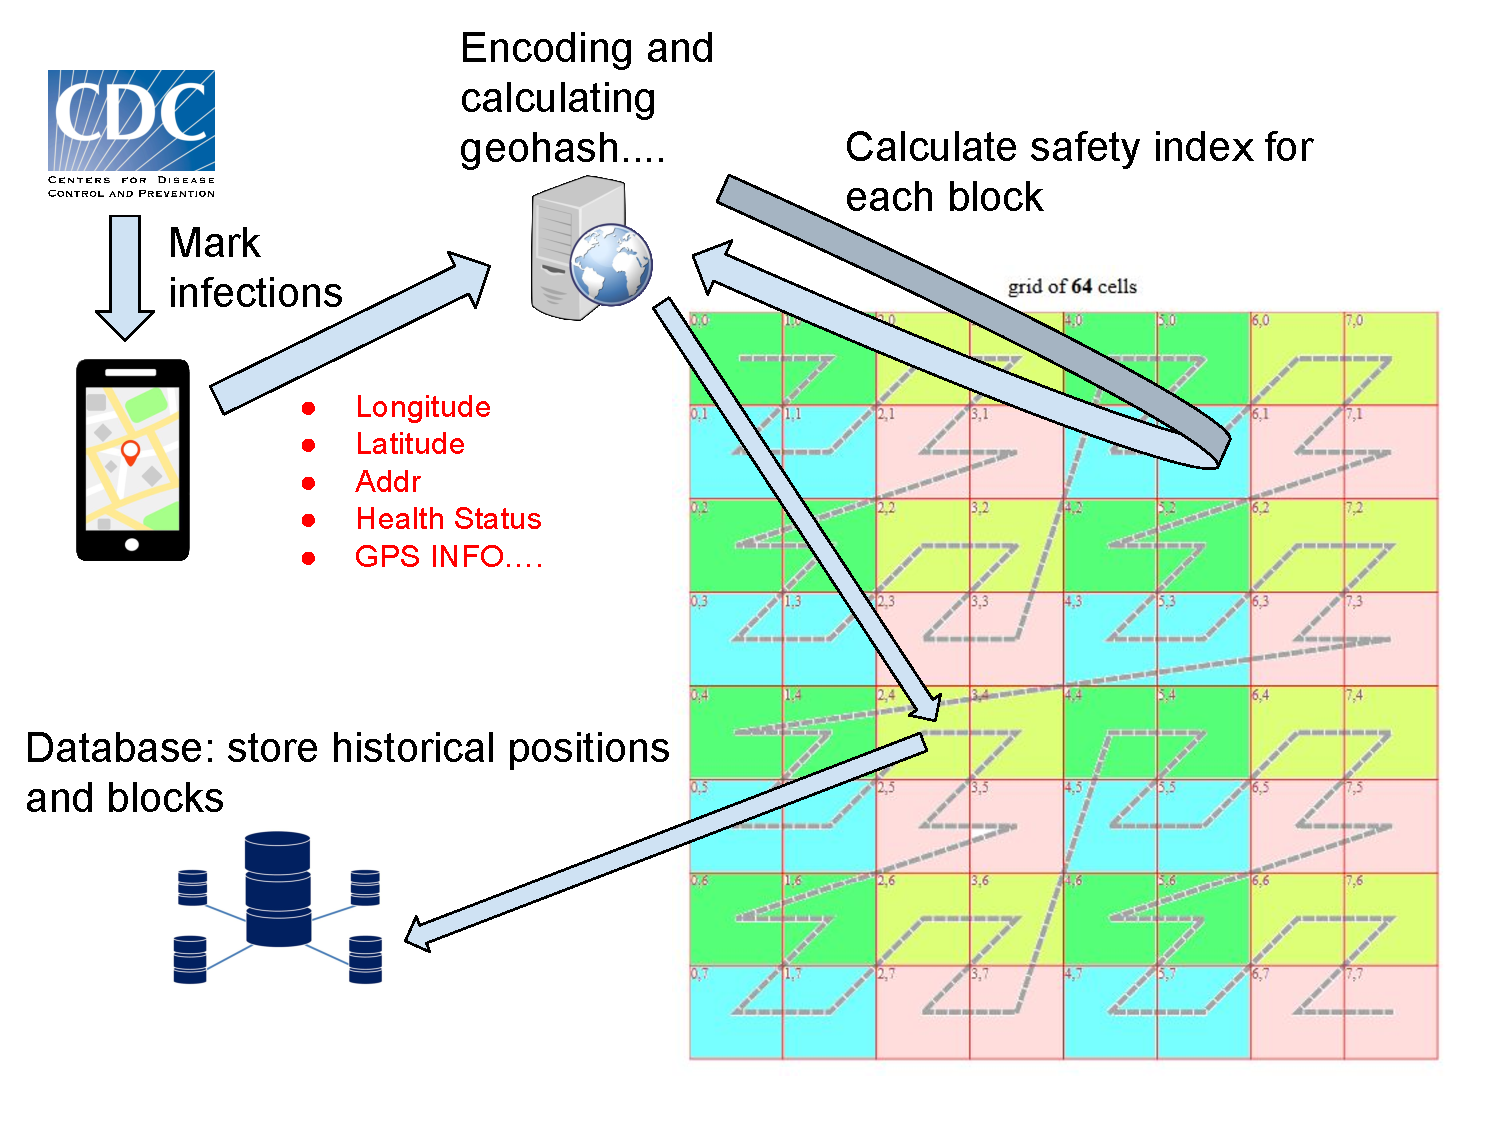
\includegraphics[width=\linewidth]{process.pdf}
	\caption{The process of data collection and quantification}
\end{figure}
\section{Implementation Methods}
In Pre-Work section, user position information is obtained through the mobile terminal.
The information contains some necessary data: userid, longitude and latitude, and \textbf{USI}\footnote{USI is ``User Safety Index'', a value of user's health in our system}.
Based on the above data, we can divide users into different blocks.
\subsection{Grid Division}
Our first step is to divide the earth into blocks or grids. \textbf{GeoHash} technology can help us achieve this step.
\textbf{GeoHash} can perform the following operations:
\begin{itemize}
	\item \textbf{GeoHash} divides a two-dimensional map into buckets of grid according to the range of longitude and latitude.
	\item \textbf{GeoHash} encodes a geographic location (longitude and latitude) into a string of binary codes.
	\item Through the incremental operation of encoded binary code, these grids are chained to a Z-order curve as Figure 8.
\end{itemize}
How does \textbf{GeoHash} achieve the above operations?
\\
We know that the geographical range of longitude is from -180\degree\ to 180\degree\ and latitude is from -90\degree\ to 90\degree\ \cite{crossley1999guide}.
We can divide the longitude into two intervals: [-180\degree, 0\degree], [0\degree, 180\degree].
We denote the two intervals by binary number ``0'' and ``1'' respectively.
In an equivalent way, we divide the latitude into two intervals: [-90\degree, 0\degree], [0\degree, 90\degree] and denote them by ``0'' and ``1''.
\\
Then we can use ``00'', ``01'', ``10'', ``11'' to represent the four grids.
Figure 8 gives examples of ``divide the earth into 4 grids'' and ``divide the earth into 16 grids''.
But in this way, the area of each grid is very large, and the grid precision is too low.
The same way is used to further subdivide into 16, 64 grids, etc.
We get higher precision by adding the bits of \textbf{GeoHash} binary which means the earth is divided into more and smaller grids.
\begin{figure}[htb]
	\centering
	\subfigure[4 Grids]{
		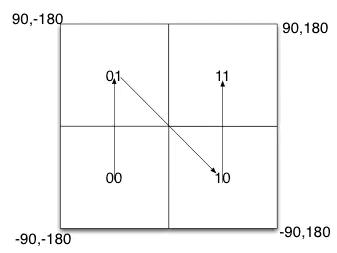
\includegraphics[width=0.45\linewidth,height=33mm]{4-grids.png}
	}
	\subfigure[16 Grids]{
		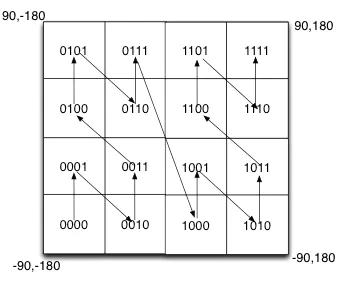
\includegraphics[width=0.45\linewidth,height=33mm]{16-grids.png}
	}
	\caption{Z-order curve to show \textbf{GeoHash} grids division}
\end{figure}
\subsection{Gird Size}
%%In addition, we found that these grids can be strung to an z-order curve, which means we can store the two-dimensional map grids in a one-dimensional array.
%%Any user shall belong to a grid.
Table 1 compares the real-world geographical distance and the length of \textbf{GeoHash} bits, the latitude is around 30\degree.
\begin{table}[htb]
	\caption{Comparison table of \textbf{GeoHash} bits and estimated geographical length of one grid}
	\begin{tabular}{lll}
		\toprule
		East-West Length(m) & South-North Length(m) & Bits \\
		\midrule
		32.67               & 19.05                 & 20*2 \\
		65.34               & 38.1                  & 19*2 \\
		130.68              & 76.2                  & 18*2 \\
		261.36              & 152.4                 & 17*2 \\
		522.72              & 304.8                 & 16*2 \\
		1045.44             & 609.6                 & 15*2 \\
		2090.88             & 1219.2                & 14*2 \\
		4181.76             & 2438.4                & 13*2 \\
		8363.52             & 4876.8                & 12*2 \\
		16727.04            & 9753.6                & 11*2 \\
		33454.08            & 19507.2               & 10*2 \\
		66908.16            & 39014.4               & 9*2  \\
		133816.32           & 78028.8               & 8*2  \\
		267632.64           & 156057.6              & 7*2  \\
		535265.28           & 312115.2              & 6*2  \\
		1070530.56          & 624230.4              & 5*2  \\
		2141061.12          & 1248460.8             & 4*2  \\
		4282122.24          & 2496921.6             & 3*2  \\
		8564244.48          & 4993843.2             & 2*2  \\
		17128488.96         & 9987686.4             & 1*2  \\
		\bottomrule
	\end{tabular}
\end{table}
Since the geometric shape of the earth is a sphere, even with the same \textbf{GeoHash} bit, the grids of high latitude contains less geographical length than those of low latitude.
Attention: the length data in Table 1 is generated from the grids around 30\degree\ latitude, it doesn't represent all the grids or an average value.
\\
Use the following formulas (1) and (2) to estimate the length of the two edges of a grid and it assumes the earth is completely spherical.
We use $G_{NS}$ to represent the length of north-south edge and $G_{EW}$ to represent the length of east-west edge as they are stroked in Figure 9.
The index $geobit$ is the length of total \textbf{GeoHash} bits which is used to represent a grid.
The length of a meridian which is $L_{meridian}$ in Formula (1) has been estimated at 20,003.93 km (12,429.9 miles) on a modern ellipsoid model of the earth (WGS 84)\cite{weintrit2013so}.
The length of the equator which is $L_{equator}$ in Formula (2) is about 40,075 km (24,901 miles) long\cite{equator2011}.
Formula (1) is used to estimate the length of the north-south edge of a grid.
Formula (2) is used to estimate the length of the east-west edge of a grid at latitude $\varphi$.
\begin{equation}
	G_{NS}\approx\frac{L_{meridian}}{2^{geobit/2}}
\end{equation}
\begin{equation}
	G_{EW}(\varphi)\approx\frac{L_{equator}\times\cos(\varphi)}{2^{geobit/2}}
\end{equation}
\\
The reason why the word ``estimate'' is used when caculating $G_{NS}$ and $G_{EW}$ here is that the earth is actually elliptical.
Earth ellipsoid will cause the following two issues:
\begin{itemize}
	\item The meridian and equator are different in length, grids at different latitudes own different $G_{NS}$ values.
	\item If the precision of the grid is not high enough, the grid is not a rectange, two different $G_{EW}$ values will appear in one grid.
\end{itemize}
In fact, under the same \textbf{GeoHash} bits, whether it is ``Earth Ellipsoid'' or ``Earth Spheroid'', the length of the two edges of a grid depends only on latitude.
If we need the accurate length of the two edges, we should start a deep discussion about ``Length of a degree of longitude'' and ``Length of a degree of latitude'', which are beyond the research scope of this paper.
Here we list our final calculation formulas when the earth is modelled by an ellipsoid, this is much more complicated but accurate than the spherical earth.
\begin{equation}
	a=\frac{L_{equator}}{2\pi}\quad b=\frac{L_{meridian}}{2\pi}
\end{equation}
\begin{equation}
	f=\frac{a-b}{a}\quad e^2=f(2-f)
\end{equation}
\begin{equation}
	\bigtriangleup\varphi=\frac{180}{2^{geobit/2}}
\end{equation}
\begin{equation}
	G_{EW}(k)=\frac{2\pi a\cos(k\Delta\varphi)}{2^{geobit/2}\sqrt{1-e^2\sin^2k\Delta\varphi}}
\end{equation}
\begin{equation}
	G_{NS}(k)=a(1-e^2)\int_{k\Delta\varphi}^{(k+1)\Delta\varphi}\frac{\operatorname d\phi}{{(1-e^2\sin^2\phi)}^\frac32}
\end{equation}
\begin{equation}
	k\in\{-2^{geobit/2-1}, -2^{geobit/2-1}+1, \ldots, 2^{geobit/2-1}-1\}
\end{equation}
\begin{figure}[htb]
	\centering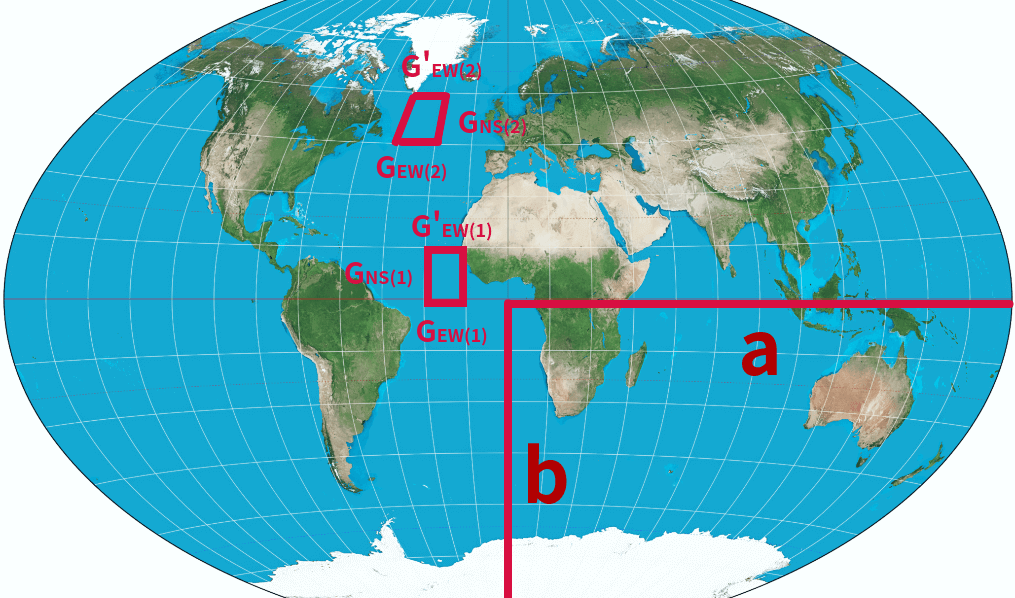
\includegraphics[width=\linewidth]{earth.png}
	\caption{Grid of elliptical earth}
\end{figure}
\\
Formula (3), (4), (5), (6), (7) and (8), give the methods to estimate the grid size of eplliptical earth.
They are used to calculate the length of each side of a grid.
The formulas are derived from \textit{The Mercator Projections}\cite{osborne2013mercator}.
Any \textbf{GeoHash} grid in our GIS has 3 different side lengths, which are represented by $G_{NS}(k)$, $G_{EW}(k)$ and $G_{EW}(k+1)$ respectively.

\subsection{Block Storage}
We store all these blocks and user data in common databases on the server.
Data storage includes two main parts:
\begin{enumerate}
	\item user historical location data
	\item block data
\end{enumerate}
One block contains many users, and one user has many position logs.
Block and user information are bidirectional associated, which is called “many to many” in the field of computer data storage model.
This section will discuss the data storage models and algorithms.
\\
Before storing the block, we have to encode the position by \textbf{GeoHash}.
The first step is to transform longitude and latitude to binary code.
Referring to the description about grid division in Section 4.1, we adopt the following Algorithm 1.
\\
\begin{algorithm}[htb]
	\caption{Transform position to GeoHash bit}
	\begin{algorithmic}[1]
		\Require{$longitude,latitude,bit$, bit is the length of GeoHash}
		\Ensure{Integer array, GeoHash binary code}
		\Function{geohash}{$longitude,latitude,bit$}
		\State{$result=[]$}
		\State{$i=0$}
		\State{$lat[0]=-90$}
		\State{$lat[1]=90$}
		\State{$lon[0]=-180$}
		\State{$lon[1]=180$}
		\While{$i<bit*2$}
		\State{$mid=(lon[0]+lon[1])/2$}
		\If{$mid>longitude$}
		\State{$result[i++]=0$}
		\State{$lon[1]=mid$}
		\Else
		\State{$result[i++]=1$}
		\State{$lon[0]=mid$}
		\EndIf
		\State{$mid=(lat[0]+lat[1])/2$}
		\If{$mid>latitude$}
		\State{$result[i++]=0$}
		\State{$lat[1]=mid$}
		\Else
		\State{$result[i++]=1$}
		\State{$lat[0]=mid$}
		\EndIf
		\EndWhile
		\State{\Return{$result$}}
		\EndFunction
	\end{algorithmic}
\end{algorithm}
\\
In the section 4.1 we have discussed that a \textbf{GeoHash} binary code can be divided into two parts: longitude part and latitude part, and they have the same number of bits in a \textbf{GeoHash} binary code.
In Algorithm 1, longitude and latitude are rankded one by one.
For example: in a returned \textbf{GeoHash} binary code, the first bit represents the range of longitude, then the second bit represents the range of latitude, and the third bit is longitude again, and so on.
This is for code simplicity, theoretically, as long as the encoding and decoding rules are consistent, how to sort \textbf{GeoHash} binary codes is not the most important thing here.
\\
If we directly save the \textbf{GeoHash} binary code of a block, a string of binary code is too long.
In the practical production environment, we do convert binary code to hexadecimal code and store the ``hex code'' in the non-relational database.
Therefore, a string of hex code can represent a block, and also it contains a range of positions.
Figure 10 shows the complete process of ``From position to \textbf{GeoHash} hex code''.
\\
When a position needs to be determined, hexadecimal code can be easily converted to binary code, and then the binary code can be decoded to the range of longitude and latitude by inversing \textbf{GeoHash} algorithm.
The accuracy of restored position depends on the number of \textbf{GeoHash} bits.
In this project, we choose 10 to 20 bits \textbf{GeoHash} to encode longitude and latitude respectively, so the total length of a generated \textbf{GeoHash} binary is 20 to 40 bits.
In the practical test, we consider such sizes of block are the most reasonable observation range for medical workers.
Thanks to the flexibility of the algorithm, we can adjust it according to the requirements.
\\
Figure 10 has illustrated the storage data structure in the non-relational database.
Hashes are maps between string keys and string values.
We set the user IDs as keys and user health information as values in a hash table.
In the database, one block corresponds to one hash table, and the hexadecimal code of block is the name of hash table.
\begin{figure}[htb]
	\centering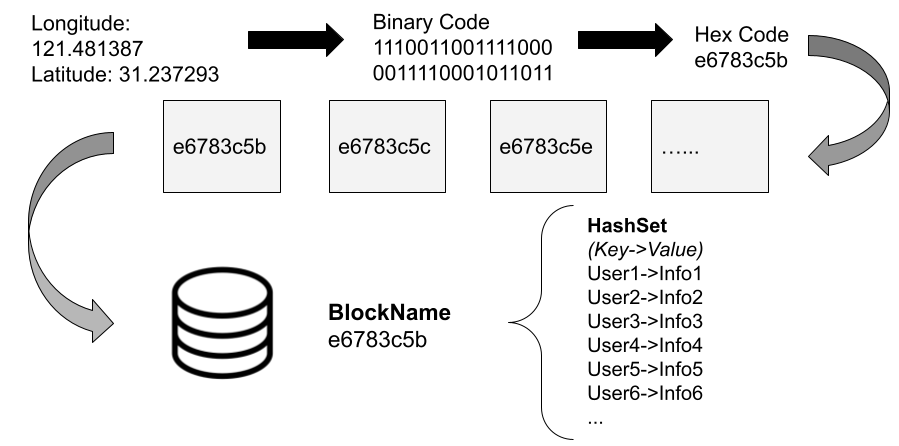
\includegraphics[width=\linewidth]{block-storage.png}
	\caption{The process of block storage}
\end{figure}
\\
In this way, when a user enters a block, a user ID and information as a ``key-value'' pair will be added to the hash table.
When the user changes the position and enters another block, the user will be moved out of the current hash table and then into the hash table of the new block.
\\
For those blocks that there are no user in it, we call them \textbf{``Depopulated Blocks''}.
These blocks are logically existed, but they are not physically stored.
By clearing the \textbf{``Depopulated Blocks''}, we free the storage space.
In contrast, when a user appears in a depopulated block, a new block will be created dynamically in the storage space, which means a new related hash table will be generated, and the user's information will be saved in the table.
\\
For the blocks that the user has entered historically, these block logs can be recorded in a relational database table at the row level.
The users' IDs are the foreign keys in the table.
When these block logs are queried from the database, as Figure 11, these blocks are organized as nodes in a link or an array following the user.
We call them \textbf{``User GeoHash Block Chain''}, \textbf{UGBC} for short.
For a block node in a link, the closer to the current time the user has entered, the more ahead in this link, the blocks that the user entered ealier will be placed at the tail of the link.
\begin{figure}[htb]
	\centering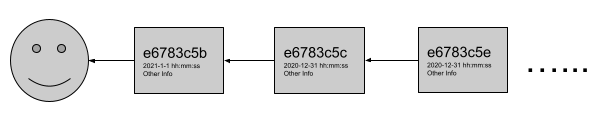
\includegraphics[width=\linewidth]{block-log.png}
	\caption{User GeoHash Block Chain}
\end{figure}
\\
COVID-19 requires us to query the past 14-days records which will generate a 14-days \textbf{UGBC}.
It is worth noting that the COVID-19 14-days \textbf{UGBC} will be used in the next section for block quantitative analysis.

\subsection{Block Quantification}
For quantitative analysis of a block, the data we need to use include the current data and the past $n$ days historical data of a block.
The ``14 days'' is for the example of COVID-19 because studies have shown that the longest incubation period of the virus is 14 days\cite{lauer2020incubation}.
\\
The sample of quantitative analysis described in this paper is to obtain a value \textbf{ASI} (Area Safety Index).
\textbf{ASI} is one of the most important indexes in our study, which reflects the safety degree of a block.
The safety degree can be calculated to a meaningful and definite quantity with \textbf{ASI}.
The following is an introduction about calculating \textbf{ASI} of a block.
The following method is considered as our ``Basic ASI Model''
\begin{equation}
	RI_n=\sum_{i=1}^n\left(\frac{R_d^iP_d}{R_o^i+R_w^i+R_d^i}+\frac{R_w^iP_w}{R_o^i+R_w^i+R_d^i}\right)P_i
\end{equation}
\begin{equation}
	ASI_{cov19}=100-RI_{14}
\end{equation}
In Formula (9), $RI$ (Risk Index) represents the past $n$ days risk index of a block.
$R_d$, $R_w$ and $R_o$ are respectively the number of confirmed cases, suspected cases, and healthy cases.
So Formula (9) actually is a risk assessment by calculating the density of infected and suspected cases in a block.
Suspected cases refer to those who have symptoms of infection, or have been in contact with confirmed cases, or have visited other high-risk blocks.
We define the blocks with \textbf{ASI} less than 60 as high-risk blocks, and the standard of high-risk can be customized in the system.
Variable $i$ counts the backtracking days.
For example, ``$i=n$'' indicates today, ``$i=n-1$'' indicates yesterday, until ``$i=1$'' is the first backtracking day, the total is $n$ days.
$P_d$ is the weight of infected cases and $P_w$ is the weight of suspected cases.
$P_i$ is the weight of time influence, the unit of time is ``day''.
Normally, the larger the day $i$ is, the higher the $P_i$ is.
\\
Constants $P_i$, $P_d$, $P_w$ need to be fitted according to the population in a block.
The calculation of $P_i$ is in Formula (11).
\begin{equation}
	P_i=\frac{100i}{(n+1)n/2}
\end{equation}
\\
The time weight $P_i$ increase linearly with the increase of day $i$.
$n$ is a constant and it is the number of backtracking days in ASI calculation.
\\
\section{Experiments}
Two groups of experiments are carried out on the block with large population and the block with small population.
The collective conditions of the two experiments for calculating ASI are:
\begin{enumerate}
	\item Simulate confirmed cases, suspected cases within 42 days.
	\item The backtracking time is 14 days, so $n=14$.
	\item If the backtrackable time is less than 14 days, set $n=i$.
	\item The total population in a block fluctuates up and down within a range.
	\item Upon ASI decreases to 60, the block will trigger lockdown, the population stops flowing in or out.
\end{enumerate}
We use \textbf{Apache Echart}\footnote{https://echarts.apache.org/examples/en/editor.html?c=mix-line-bar} to visualize the experimental results.
In Figure 12, the red line is the cordon of lockdown which also means under it is a high-risk period.
When \textbf{ASI} touches the red line, we think it is necessary to take lockdown or other effective measures.
The yellow line represents the trend of \textbf{ASI}.
The blue bar indicates the number of confirmed cases and the green bar indicates the number of suspected cases.
Both of the confirmed and suspected cases increase from day 1, and decrease after reaching the peak until 0.

\subsection{Small Population}
For small population block, we assume the following conditions:
\begin{enumerate}
	\item The population range is $[500,1000]$ in a block.
	\item $P_d=45$ and $P_w=15$.
\end{enumerate}
The experimental results of small population block have been plotted as shown in Figure 12, ``Small population''.
When the confirmed cases and suspected cases increaes, \textbf{ASI} decreases.
\textbf{ASI} decreases to $46.47$ on day 10 and drops to $0$ on day 15.
Until day 31, \textbf{ASI} returns to above 60.
So we can set the block in high-risk from day 10 to 31.

\subsection{Large Population}
For large population block, we assume the following conditions:
\begin{enumerate}
	\item The population range is $[960000,1000000]$ in a block.
	\item $P_d=8000$ and $P_w=4000$.
\end{enumerate}
The experimental results of large population block have been plotted as shown in Figure 12, ``Large population''.
From the ``Large population'' chart, \textbf{ASI} decreases to $47.35$ on day 13 and goes back to $68$ on day 27.
Then we set the block in high-risk from day 13 to 27.

\begin{figure*}[hptb]
	\centering{
		\subfigure[Small population]{
			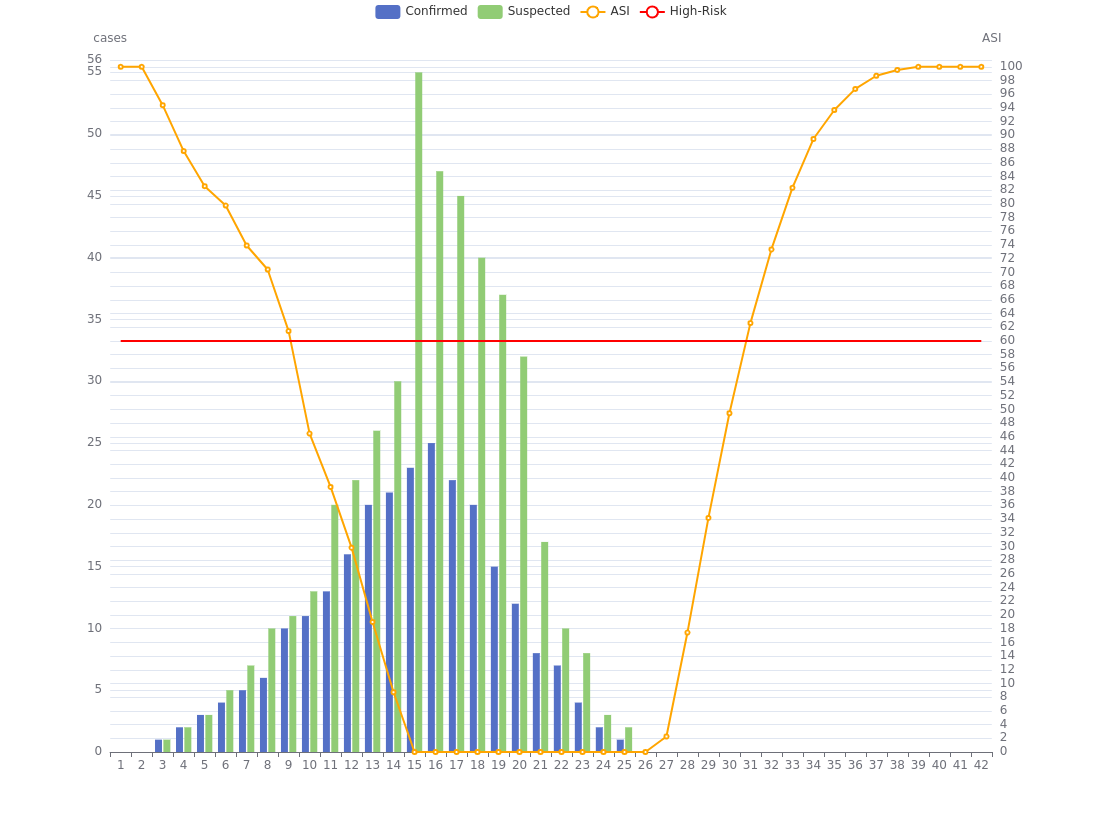
\includegraphics[width=16cm,height=10.5cm]{echarts-sm.png}
		}
		\subfigure[Large population]{
			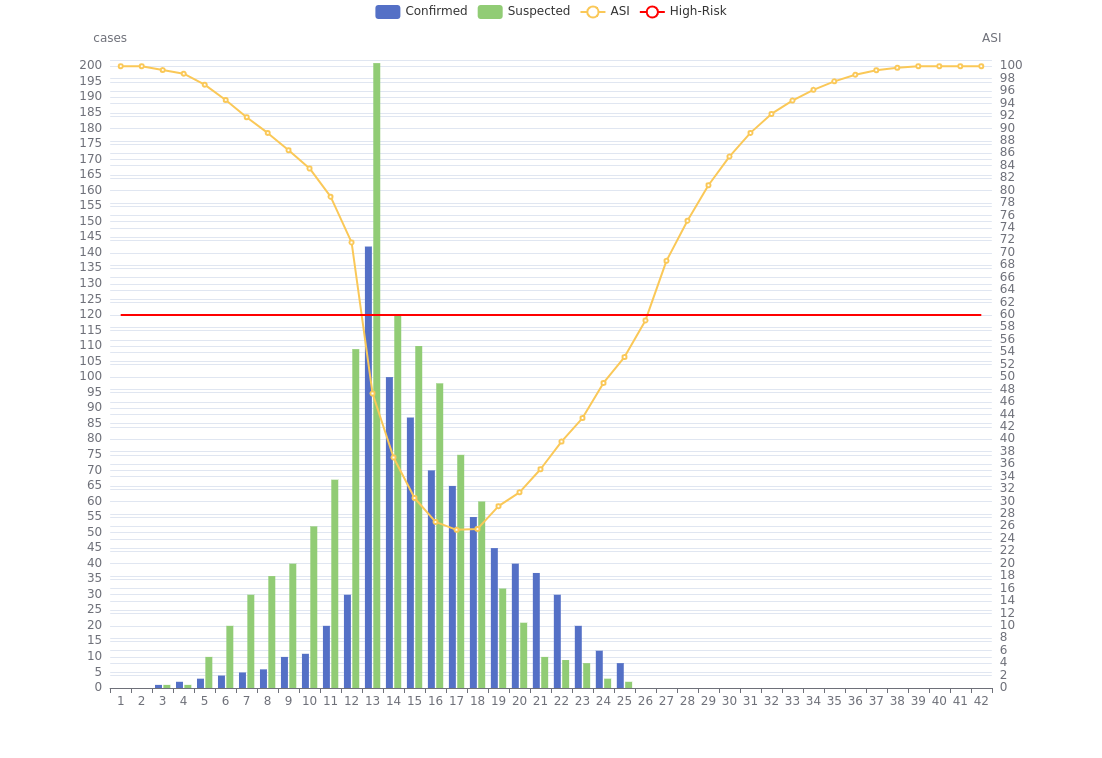
\includegraphics[width=16cm,height=10.5cm]{echarts-lg.png}
		}
		\caption{Experimental results charts}
	}
\end{figure*}
\newpage

\section{Conclusions}
The conclusion is
\section{Future Work}
In addition to \textbf{ASI}, we can also conduct other types of data analysis based on \textbf{GeoHash} blocks, and get more useful results to help us carry out epidemic prevention and control.
Such as the medical level of a block, and even predict the possibility value of an epidemic outbreak in a block.
These are the directions that can be studied based on \textbf{GeoHash} blocks, and we are working on these studies.
\\
Algorithms will be improved by following the new progress of medical research to handle the changing pandemic.
We need to take more interdisciplinary cooperation, especially in infectious disease medicine and bioinformatics.
Medical professionals can help us to find more suitable risk assessment models and algorithms on \textbf{GeoHash}.
\\
Considering the similarity of data structure, we are trying to use blockchain technology to decentralize the storage and calculation of epidemic data.
We note that other international research teams have also carried out research on blockchain using for health care domain.\cite{nguyen2020blockchain}\cite{CryptocurrencyNewUse2020Coronavirus}
Blockchain technology can help us reduce the pressure of central storage, protect the privacy of users through anonymity\cite{nakamoto2019bitcoin}, and ensure that the data can not be tampered.\cite{armstrong2016move}
\bibliographystyle{unsrt}
\bibliography{refs}
\end{document}
\endinput
